\documentclass[12pt]{jarticle}

\usepackage[dvipdfmx]{graphicx}
\usepackage{url}
\usepackage{listings,jlisting}
\usepackage{ascmac}
\usepackage{amsmath,amssymb}
\usepackage{comment}

%ここからソースコードの表示に関する設定
\lstset{
  basicstyle={\ttfamily},
  identifierstyle={\small},
  commentstyle={\smallitshape},
  keywordstyle={\small\bfseries},
  ndkeywordstyle={\small},
  stringstyle={\small\ttfamily},
  frame={tb},
  breaklines=true,
  columns=[l]{fullflexible},
  numbers=left,
  xrightmargin=0zw,
  xleftmargin=3zw,
  numberstyle={\scriptsize},
  stepnumber=1,
  numbersep=1zw,
  lineskip=-0.5ex
}
%ここまでソースコードの表示に関する設定

\title{知能プログラミング演習II 課題5}
\author{グループ8\\
  29114142 湯浅範子\\
}
\date{2019年12月3日}

\begin{document}
\maketitle

\paragraph{提出物} rep5(2914142.pdf),group08.zip
\paragraph{グループ} グループ8
\paragraph{メンバー}
\begin{tabular}{|c|c|c|}
  \hline
  学生番号&氏名&貢献度比率\\
  \hline\hline
  29114003&青山周平&\\
  \hline
  29114060&後藤拓也&\\
  \hline
  29114116&増田大輝&\\
  \hline
  29114142&湯浅範子&\\
  \hline
  29119016&小中祐希&\\
  \hline
\end{tabular}

\section{課題の説明}
\begin{description}
\item[必須課題5-1] 目標集合を変えてみたときに,動作が正しくない場合があったかどうか,実行例を示して考察せよ.
また,もしあったならその箇所を修正し,どのように修正したか記せ.
\item[必須課題5-2] 教科書のプログラムでは,オペレータ間の競合解消戦略としてランダムなオペレータ選択を採用している.
これを,効果的な競合解消戦略に改良すべく考察し,実装せよ.
改良の結果,性能がどの程度向上したかを定量的に(つまり数字で)示すこと.
\item[必須課題5-3] 上記のプランニングのプログラムでは,ブロックの属性(たとえば色や形など)を考えていないので,色や形などの属性を扱えるようにせよ.ルールとして表現すること.
例えば色と形の両方を扱えるようにする場合,Aが青い三角形,Bが黄色の四角形,Cが緑の台形であったとする.
その時,色と形を使ってもゴールを指定できるようにする("green on blue" や"blue on box"のように)
\item[必須課題5-4] 上記5-2, 5-3で改良したプランニングシステムのGUIを実装せよ.
ブロック操作の過程をグラフィカルに可視化し,初期状態や目標状態をGUI上で変更できることが望ましい.
\item[発展課題5-5] ブロックワールド内における物理的制約条件をルールとして表現せよ.
例えば,三角錐(pyramid)の上には他のブロックを乗せられない等,その世界における物理的な制約を実現せよ.
\item[発展課題5-6] ユーザが自然言語(日本語や英語など)の命令文によってブロックを操作したり,初期状態/目標状態を変更したりできるようにせよ.
なお,命令文の動詞や語尾を1つの表現に決め打ちするのではなく,多様な表現を許容できることが望ましい.
\item[発展課題5-7] 3次元空間 (実世界) の物理的な挙動を考慮したブロックワールドにおけるプランニングを実現せよ.
なお,物理エンジン等を利用する場合,Java以外の言語のフレームワークを使って実現しても構わない.
\item[発展課題5-8] 教科書3.3節のプランニング手法を応用できそうなブロック操作以外のタスクをグループで話し合い,新たなプランニング課題を自由に設定せよ.
さらに,もし可能であれば,その自己設定課題を解くプランニングシステムを実装せよ.
\end{description}
私は必須課題5-4のGUI実装を行ったため,それについて記述する.

\section{必須課題5-4}
\begin{screen}
  上記5-2, 5-3で改良したプランニングシステムのGUIを実装せよ.\par
ブロック操作の過程をグラフィカルに可視化し,初期状態や目標状態をGUI上で変更できることが望ましい.
\end{screen}
私の担当箇所は,得られた結果を基にしたGUI本体の実装である.

\subsection{手法}
GUIで求められる出力が行えるように,以下のような機能を加えた.

\begin{itemize}
\item ブロック操作の過程を示す
\item ブロック操作の過程をグラフィカルに可視化する
\item 初期状態と目標状態をGUI上から自然言語で変更できる
\item 属性の決定をGUI上から行える
\item 操作に必要なオペレータと属性のデータを表示する
\end{itemize}

これらのプログラムを実装するためのデータ受け渡し部分は青山君が作成してくれるため,ここでは受け取ったデータを基にしてどのような方法で表示を行うかを考えながら実装を行った.\\

また今回は初めてのGUI作成であったため,データの受け渡し部分の作成を待つ間に,データを既に得ていると仮定した仮データを基にしてGUIの検討を行った.\\

\subsection{実装}
今週は仮のデータを基にどのようにしてGUIを作成するかを考えたため,それに関する実装を以下に示す.

まず,ブロック操作の過程をグラフィカルに可視化するために,CardLayoutを用いてブロック状態の変化の実装を行うこととした.これに関するプログラムをソースコード\ref{CardLayout}に示す.
\begin{lstlisting}[caption=CardLayout関連プログラム,label=CardLayout]
// 切り替え用ページの設定
ArrayList<JPanel> card = new ArrayList<>();
// ページの追加(必要ページ数分だけ繰り返す)
card.add(new JPanel()); 
card.get(0).add(page1);
// パネルの設定
cardPanel = new JPanel();
layout = new CardLayout();
cardPanel.setLayout(layout);

cardPanel.add(card.get(0), "start");
cardPanel.add(card.get(1), "label1");
・・・
cardPanel.add(card.get(card.size()-1), "finish");

// カード移動用ボタン
JButton firstButton = new JButton("First");
firstButton.addActionListener(this);
firstButton.setActionCommand("First");
JButton prevButton = new JButton("Prev");
prevButton.addActionListener(this);
prevButton.setActionCommand("Prev");
JButton nextButton = new JButton("Next");
nextButton.addActionListener(this);
nextButton.setActionCommand("Next");
JButton lastButton = new JButton("Last");
lastButton.addActionListener(this);
lastButton.setActionCommand("Last");

// カード遷移設定ボタンを一列の画面に
JPanel btnPanel = new JPanel();
btnPanel.add(firstButton);
btnPanel.add(prevButton);
btnPanel.add(nextButton);
btnPanel.add(lastButton);

// カード移動用ボタンの動作設定
public void actionPerformed(ActionEvent e){
	// 画面遷移用
	String cmd = e.getActionCommand();
	if (cmd.equals("First")){
		layout.first(cardPanel);
	}else if (cmd.equals("Last")){
		layout.last(cardPanel);
	}else if (cmd.equals("Next")){
		layout.next(cardPanel);
	}else if (cmd.equals("Prev")){
		layout.previous(cardPanel);
	}
}
\end{lstlisting}
状態遷移をグラフィカルに可視化するため,CardLayoutを用いた.これにより任意の数だけ状態遷移画面を作成でき,それらが全てボタンによって移動できるようになっている.さらにカードの一番初めと一番最後に移動するためのボタンを作成したことにより,いつでも初期画面に戻ることが出来る.

次に,実際にブロック操作の状態を表すためのプログラムをソースコード\ref{page2}に示す.
\begin{lstlisting}[caption=ブロックの状態を表すプログラム,label=page2]
// 結果表示用ページで共通の変数
row = 4;
col = 3;
ImageIcon arm = new ImageIcon("arm't.png");
ImageIcon icon1 = new ImageIcon("sanRt.png");
ImageIcon icon2 = new ImageIcon("enGt.png");
ImageIcon icon3 = new ImageIcon("squBt.png");
String armname = "   ";
String icon1name = "A";
String icon2name = "B";
String icon3name = "C";
String no = "";
// 新規ページの作成
card.add(new JPanel());
JPanel page2 = new JPanel();
JLabel[][] p2Label = new JLabel[row][col];
page2.setPreferredSize(new Dimension(row*80, col*80));
page2.setBackground(Color.WHITE);
GridLayout page2layout = new GridLayout();
page2layout.setRows(row); // 行数
page2layout.setColumns(col); // 列数
page2.setLayout(page2layout);
// 中身の設定(2ページ)
p2Label[0][0] = new JLabel(no);
p2Label[0][1] = new JLabel(arm);
p2Label[0][1].setText(armname);
p2Label[0][2] = new JLabel(no);
p2Label[1][0] = new JLabel(no);
p2Label[1][1] = new JLabel(no);
p2Label[1][2] = new JLabel(no);
p2Label[2][0] = new JLabel(no);
p2Label[2][1] = new JLabel(no);
p2Label[2][2] = new JLabel(no);
p2Label[3][0] = new JLabel(icon1);
p2Label[3][0].setText(icon1name);
p2Label[3][1] = new JLabel(icon2);
p2Label[3][1].setText(icon2name);
p2Label[3][2] = new JLabel(icon3);
p2Label[3][2].setText(icon3name);
for (int i = 0; i < row; i++) {
	for (int j = 0; j < col; j++) {
		page2.add(p2Label[i][j]);
	}
}
// 出力結果(各ステップ)の表示
JPanel list = new JPanel();
list.setLayout(new BoxLayout(list, BoxLayout.PAGE_AXIS));
for (int i = 0; i < results.size(); i++) {
	JLabel now = new JLabel(results.get(i));
	if (i == 0) {
		now.setBackground(Color.ORANGE);
		now.setOpaque(true);
	}
	list.add(now);
	if (i == results.size()-1) {
		list.add(new JLabel(" "));
		list.add(new JLabel(" "));
	}
}
card.get(1).add(list);
card.get(1).add(page2);
\end{lstlisting}
ブロックの状態を表すため,BoxLayoutを用いて実装を行った.表示する図形については,新たに作成したpngファイルにあらかじめ図形を描き,これをアイコンとして挿入することでGUI上での描画を行った.さらに,現在行われている描画が操作手順のどこに当たるのかを,全体の出力結果を用いて表した.

次に,初期状態と目標状態,属性の決定を行うためのプログラムをソースコード\ref{page1}に示す.
\begin{lstlisting}[caption=初期状態と目標状態,属性の決定,label=page1]
// 初期状態選択画面
card.add(new JPanel()); // ページの追加
// 選択用ラジオボタンパネル
JPanel allRadio = new JPanel();
allRadio.setLayout(new BoxLayout(allRadio, BoxLayout.PAGE_AXIS));
// 色選択
JPanel p2 = new JPanel();
p2.setLayout(new BoxLayout(p2, BoxLayout.PAGE_AXIS));
radio = new JRadioButton[4];
radio[0] = new JRadioButton("Blue");
radio[1] = new JRadioButton("Green");
radio[2] = new JRadioButton("Red");
radio[3] = new JRadioButton("Yellow");
// ボタンのグループ化
ButtonGroup group = new ButtonGroup();
group.add(radio[0]);
group.add(radio[1]);
group.add(radio[2]);
group.add(radio[3]);
p2.add(new JLabel("Select Color"));
p2.add(radio[0]);
p2.add(radio[1]);
p2.add(radio[2]);
p2.add(radio[3]);
// 形状選択(色選択と同様の操作を行う)
・・・
// 属性決定ボタンの作成
allRadio.add(p2);
allRadio.add(Box.createRigidArea(new Dimension(10,10)));
allRadio.add(p3);
JButton set = new JButton("Set");
allRadio.add(Box.createRigidArea(new Dimension(10,10)));
allRadio.add(set);
// 属性入力用パネルの作成
JPanel attribution = new JPanel();
attribution.setLayout(new BoxLayout(attribution, BoxLayout.LINE_AXIS));
JPanel p4 = new JPanel();
p4.setLayout(new BoxLayout(p4, BoxLayout.PAGE_AXIS));
p4.add(new JLabel("Determine Attribution"));
JPanel attribute = new JPanel();
attribute.setPreferredSize(new Dimension(100, 350));
attribute.setBackground(Color.WHITE);
p4.add(attribute);
attribution.add(allRadio);
attribution.add(p4);
// 入力確認用ボタン
JPanel buttonpanel = new JPanel();
JButton button = new JButton("Search");
button.addActionListener(this);
buttonpanel.add(button);
// 手動入力用パネル
JPanel natural = new JPanel();
natural.setLayout(new BoxLayout(natural, BoxLayout.PAGE_AXIS));
// 入力(setInitialState)
JPanel sI = new JPanel();
sI.setLayout(new BoxLayout(sI, BoxLayout.PAGE_AXIS));
JLabel setInitial = new JLabel("SetInitial");
JTextArea iArea = new JTextArea(9, 20);
JScrollPane iScroll = new JScrollPane(iArea);
String ii = "";
for(String i : initialState) {
	ii += i + "\n";
}
iArea.setText(ii);
sI.add(setInitial);
sI.add(iScroll);
// 入力(setGoal)(setInitialStateと同様の操作を行う)
・・・
natural.add(sI);
natural.add(Box.createRigidArea(new Dimension(10,5)));
natural.add(sG);
JPanel page1 = new JPanel();
page1.setPreferredSize(new Dimension(500, 350));
page1.setLayout(new BorderLayout(20, 5));
page1.add(attribution, BorderLayout.LINE_START);
page1.add(natural, BorderLayout.CENTER);
page1.add(buttonpanel, BorderLayout.PAGE_END);
card.get(0).add(page1);
\end{lstlisting}
startメソッドでは,ファイルの読み込みによるルールの構築のみを行う.またfetchRulesでは現在所持しているルールをRuleBaseクラスからgetRulesメソッドで取得し返却を行うことで一覧表示が行えるようにした.\\

最後に,プログラムで使用するオペレータを表示するプログラムのソースコード\ref{Operator}のように実装した.
\begin{lstlisting}[caption=オペレータの表示,label=Operator]
// 最終ページ
card.add(new JPanel());
// オペレータの取得
ArrayList<Operator> operators = presenter.getOperatorList();
JPanel tostring = new JPanel();
tostring.setLayout(new BoxLayout(tostring, BoxLayout.PAGE_AXIS));
tostring.setBackground(Color.WHITE);
int i = 1;
for (Operator operator : operators) {
	tostring.add(new JLabel("●Operator" + i));
	tostring.add(new JLabel("NAME: " + operator.getName()));
	tostring.add(new JLabel("ADD: " + operator.getName()));
	tostring.add(new JLabel("DELETE: " + operator.getName()));
	if (i < operators.size()) {
		tostring.add(new JLabel("  "));
	}
	i++;
}
JScrollPane scrollpane = new JScrollPane(tostring);
scrollpane.setPreferredSize(new Dimension(250, 310));
BevelBorder border = new BevelBorder(BevelBorder.LOWERED);
scrollpane.setBorder(border);
// 編集用ボタン
JPanel edit = new JPanel();
edit.setLayout(new BoxLayout(edit, BoxLayout.PAGE_AXIS));
edit.add(new JButton("追加"));
edit.add(Box.createRigidArea(new Dimension(10,5)));
edit.add(new JButton("編集"));
edit.add(Box.createRigidArea(new Dimension(10,5)));
edit.add(new JButton("削除"));
JPanel tostring2 = new JPanel();
tostring2.setPreferredSize(new Dimension(200, 300));
tostring2.setBackground(Color.WHITE);
// ページへの追加
card.get(card.size()-1).add(scrollpane);
card.get(card.size()-1).add(edit);
card.get(card.size()-1).add(tostring2);
\end{lstlisting}
ここではプログラムで使用したオペレータの表示を行う.オペレータの取得は,班の人が作成してくれたオペレータ情報を取得するgetOperatorListを利用した.さらに,オペレータの編集用にボタンを作成したが,話し合いの結果プログラム中でオペレータに対しての編集は行わないこととしたため,このボタンは使用しないことになった.

\subsection{実行例}
現時点で作成したプログラムの実行結果を順に示す.\\

実行すると初めに初期状態・目標状態・属性の決定画面になる(図\ref{fig:page1}).
\begin{figure}[htbp]
  \begin{center}
    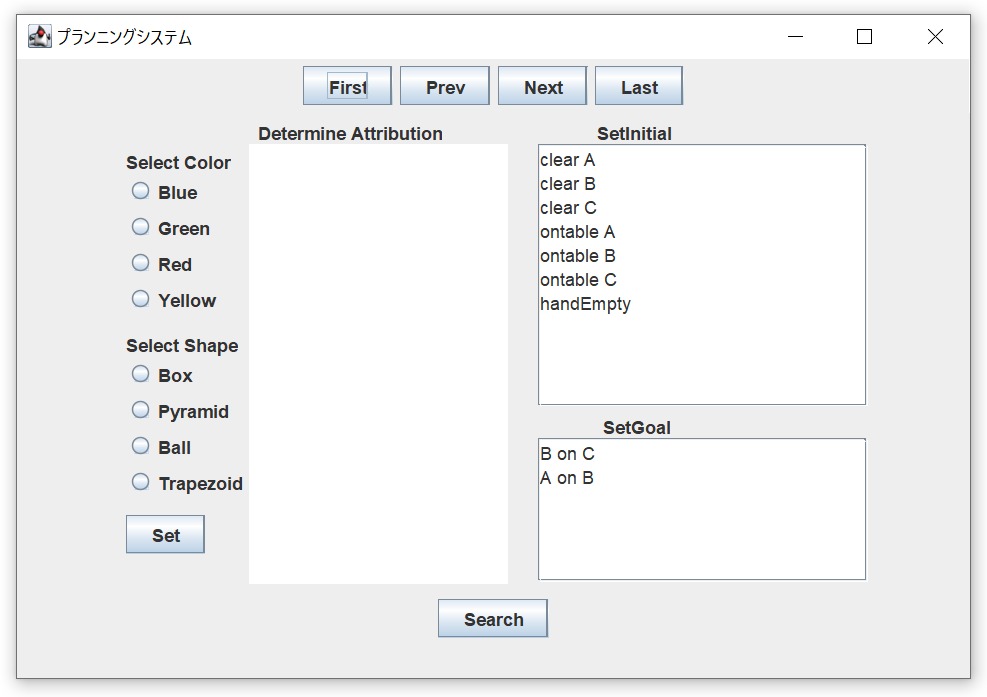
\includegraphics[scale=0.6]{images/page1.PNG}
    \caption{初期状態と目標状態,属性の決定画面}
    \label{fig:page1}
  \end{center}
\end{figure}
\clearpage
この状態でNextボタンを押すと次の画面に遷移し,ブロック操作の過程の描画画面となる.この状態でNextボタンを押すと次の状態へ,Prevボタンを押すと一つ前の状態へ遷移する様子が確認できる.(図\ref{fig:page2},次ページ図\ref{fig:page3},次ページ図\ref{fig:page6}).
\begin{figure}[htbp]
  \begin{center}
    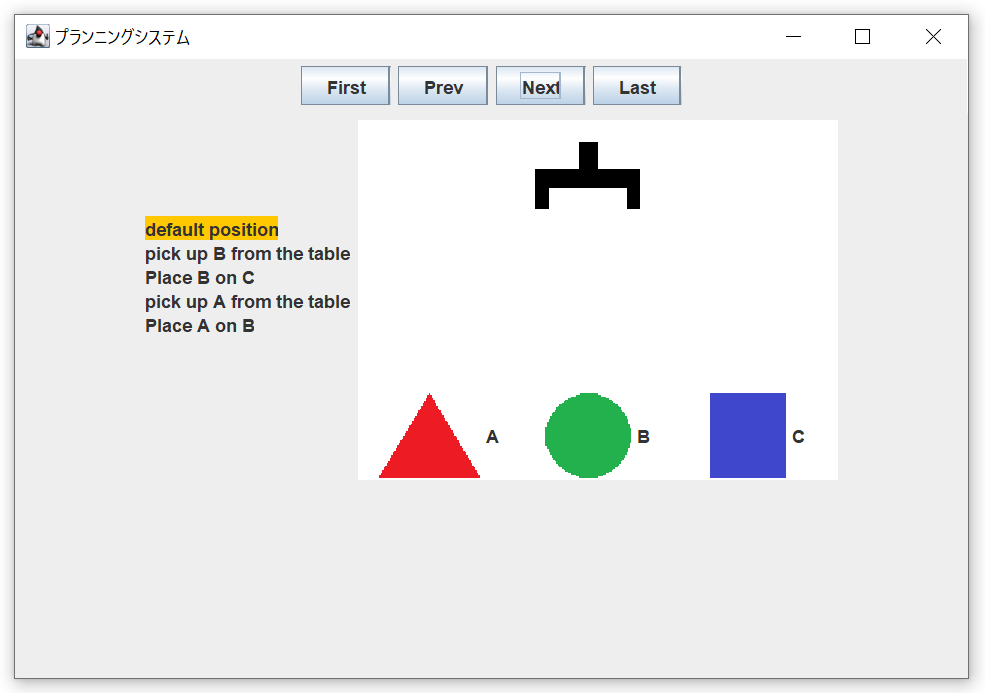
\includegraphics[scale=0.6]{images/page2.PNG}
    \caption{ブロック操作の過程1}
    \label{fig:page2}
  \end{center}
\end{figure}
\begin{figure}[htbp]
  \begin{center}
    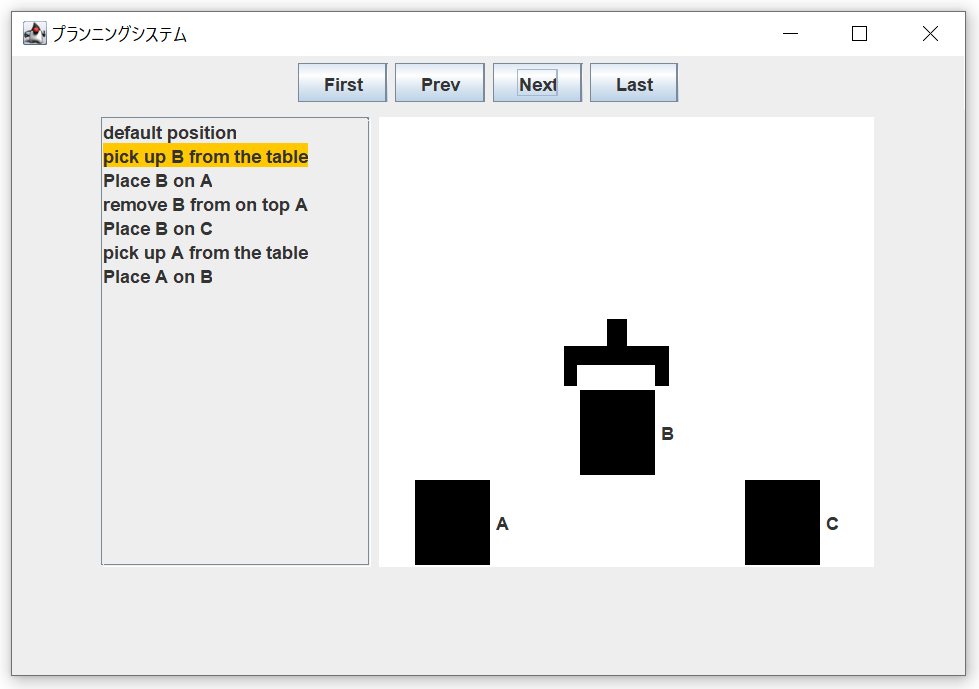
\includegraphics[scale=0.6]{images/page3.PNG}
    \caption{ブロック操作の過程2}
    \label{fig:page3}
  \end{center}
\end{figure}
\begin{figure}[htbp]
  \begin{center}
    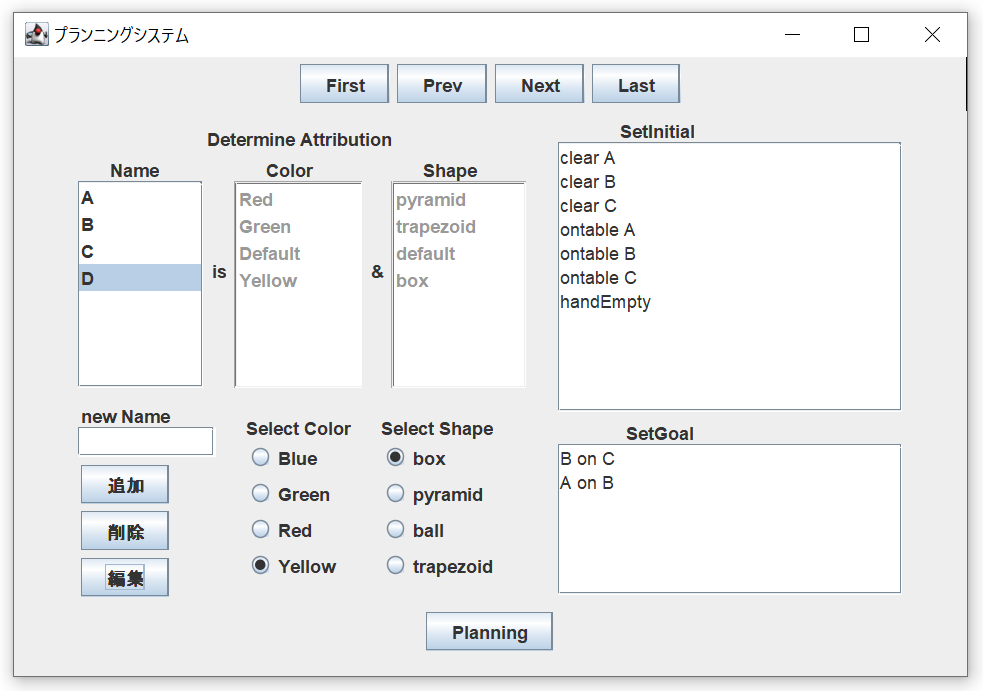
\includegraphics[scale=0.6]{images/page6.PNG}
    \caption{ブロック操作の過程3}
    \label{fig:page6}
  \end{center}
\end{figure}
\clearpage
さらにLastボタンを押すと,一番最後のページに移動することが出来,ここではオペレータの情報が示されている(図\ref{fig:page7}).
\begin{figure}[htbp]
  \begin{center}
    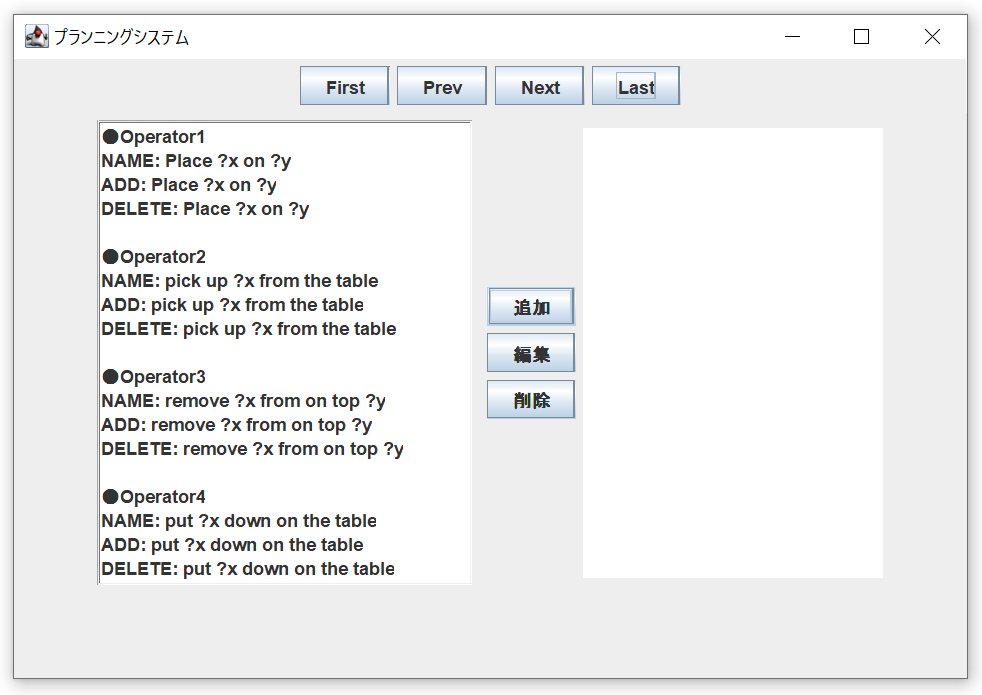
\includegraphics[scale=0.6]{images/page7.PNG}
    \caption{オペレータの情報}
    \label{fig:page7}
  \end{center}
\end{figure}
\subsection{考察}
状態遷移をグラフィカルに可視化するため,ページを移動するたびに一つずつ動作が進んでいく状態が理想であると考えた.\par
また,状態空間を描画するために,BoxLayoutで空間を座標のようにとらえることを考えた.初めはプログラム自身で図の描画を行う予定であったが,三角形などの描画は座標を指定してプログラムをしなければならず,その場合はレイアウトマネージャーを利用できなくなってしまう.これではGUIの実装が困難であるため,今回はプログラムでの図形の描画は行わないこととした.そのため,新しく自分でpng画像を作成し,これを取り込んでアイコンとして利用することで,レイアウトマネージャーを利用して図形を描画することが可能となった.\par
しかし,この方法を用いると,取り込んだ図に対して操作を行うことは出来ないことが分かった.そのため,画像の上に重なるように図形の名称(A,B,C等)を入れることや,取り込んだ画像の色を上書きすることが出来ないため,今回は図形の横に名称を記載し,画像は色違いのものをはじめから用意しておくことでこの問題を解決した.



\section{感想}
GUIは初めて作成したため慣れない部分も多く大変だったが,少し理解を深められた.\par
まだ完成には程遠いので,今週も頑張りたい.

% 参考文献
\begin{thebibliography}{99}
\bibitem{Java新} 新谷虎松『Javaによる知能プログラミング入門』コロナ社,2002年.
\bibitem{Swing} Let'sプログラミング Swingを使ってみよう, \url{https://www.javadrive.jp/tutorial/} (2019年12月3日アクセス).
\end{thebibliography}

\end{document}
